\documentclass[a4paper,twoside]{article}
% My LaTeX preamble file - by Nathaniel Dene Hoffman
% Credit for much of this goes to Olivier Pieters (https://olivierpieters.be/tags/latex)
% and Gilles Castel (https://castel.dev)
% There are still some things to be done:
% 1. Update math commands using mathtools package (remove ddfrac command and just override)
% 2. Maybe abbreviate \imath somehow?
% 3. Possibly format for margin notes and set new margin sizes
% First, some encoding packages and useful formatting
%--------------------------------------------------------------------------------------------
\usepackage{import}
\usepackage{pdfpages}
\usepackage{transparent}
\usepackage[l2tabu,orthodox]{nag}   % force newer (and safer) LaTeX commands
\usepackage[utf8]{inputenc}         % set character set to support some UTF-8
                                    %   (unicode). Do NOT use this with
                                    %   XeTeX/LuaTeX!
\usepackage[T1]{fontenc}
\usepackage[english]{babel}         % multi-language support
\usepackage{sectsty}                % allow redefinition of section command formatting
\usepackage{tabularx}               % more table options
\usepackage{booktabs}
\usepackage{titling}                % allow redefinition of title formatting
\usepackage{imakeidx}               % create and index of words
\usepackage{xcolor}                 % more colour options
\usepackage{enumitem}               % more list formatting options
\usepackage{tocloft}                % redefine table of contents, new list like objects
\usepackage{subfiles}               % allow for multifile documents

% Next, let's deal with the whitespaces and margins
%--------------------------------------------------------------------------------------------
\usepackage[centering,margin=1in]{geometry}
\setlength{\parindent}{0cm}
\setlength{\parskip}{2ex plus 0.5ex minus 0.2ex} % whitespace between paragraphs

% Redefine \maketitle command with nicer formatting
%--------------------------------------------------------------------------------------------
\pretitle{
  \begin{flushright}         % align text to right
    \fontsize{40}{60}        % set font size and whitespace
    \usefont{OT1}{phv}{b}{n} % change the font to bold (b), normally shaped (n)
                             %   Helvetica (phv)
    \selectfont              % force LaTeX to search for metric in its mapping
                             %   corresponding to the above font size definition
}
\posttitle{
  \par                       % end paragraph
  \end{flushright}           % end right align
  \vskip 0.5em               % add vertical spacing of 0.5em
}
\preauthor{
  \begin{flushright}
    \large                   % font size
    \lineskip 0.5em          % inter line spacing
    \usefont{OT1}{phv}{m}{n}
}
\postauthor{
  \par
  \end{flushright}
}
\predate{
  \begin{flushright}
  \large
  \lineskip 0.5em
  \usefont{OT1}{phv}{m}{n}
}
\postdate{
  \par
  \end{flushright}
}

% Mathematics Packages
\usepackage[Gray,squaren,thinqspace,cdot]{SIunits}      % elegant units
\usepackage{amsmath}                                    % extensive math options
\usepackage{amsfonts}                                   % special math fonts
\usepackage{mathtools}                                  % useful formatting commands
\usepackage{amsthm}                                     % useful commands for building theorem environments
\usepackage{amssymb}                                    % lots of special math symbols
\usepackage{mathrsfs}                                   % fancy scripts letters
\usepackage{cancel}                                     % cancel lines in math
\usepackage{esint}                                      % fancy integral symbols
\usepackage{relsize}                                    % make math things bigger or smaller
%\usepackage{bm}                                         % bold math!
\usepackage{slashed}

\newcommand\ddfrac[2]{\frac{\displaystyle #1}{\displaystyle #2}}    % elegant fraction formatting
\allowdisplaybreaks[1]                                              % allow align environments to break on pages

% Ensure numbering is section-specific
%--------------------------------------------------------------------------------------------
\numberwithin{equation}{section}
\numberwithin{figure}{section}
\numberwithin{table}{section}

% Citations, references, and annotations
%--------------------------------------------------------------------------------------------
\usepackage[small,bf,hang]{caption}        % captions
\usepackage{subcaption}                    % adds subfigure & subcaption
\usepackage{sidecap}                       % adds side captions
\usepackage{hyperref}                      % add hyperlinks to references
\usepackage[noabbrev,nameinlink]{cleveref} % better references than default \ref
\usepackage{autonum}                       % only number referenced equations
\usepackage{url}                           % urls
\usepackage{cite}                          % well formed numeric citations
% format hyperlinks
\colorlet{linkcolour}{black}
\colorlet{urlcolour}{blue}
\hypersetup{colorlinks=true,
            linkcolor=linkcolour,
            citecolor=linkcolour,
            urlcolor=urlcolour}

% Plotting and Figures
%--------------------------------------------------------------------------------------------
\usepackage{tikz}          % advanced vector graphics
\usepackage{pgfplots}      % data plotting
\usepackage{pgfplotstable} % table plotting
\usepackage{placeins}      % display floats in correct sections
\usepackage{graphicx}      % include external graphics
\usepackage{longtable}     % process long tables

% use most recent version of pgfplots
\pgfplotsset{compat=newest}

% Misc.
%--------------------------------------------------------------------------------------------
\usepackage{todonotes}  % add to do notes
\usepackage{epstopdf}   % process eps-images
\usepackage{float}      % floats
\usepackage{stmaryrd}   % some more nice symbols
\usepackage{emptypage}  % suppress page numbers on empty pages
\usepackage{multicol}   % use this for creating pages with multiple columns
\usepackage{etoolbox}   % adds tags for environment endings
\usepackage{tcolorbox}  % pretty colored boxes!


% Custom Commands
%--------------------------------------------------------------------------------------------
\newcommand\hr{\noindent\rule[0.5ex]{\linewidth}{0.5pt}}                % horizontal line
\newcommand\N{\ensuremath{\mathbb{N}}}                                  % blackboard set characters
\newcommand\R{\ensuremath{\mathbb{R}}}
\newcommand\Z{\ensuremath{\mathbb{Z}}}
\newcommand\Q{\ensuremath{\mathbb{Q}}}
%\newcommand\C{\ensuremath{\mathbb{C}}}
\renewcommand{\arraystretch}{1.2}                                       % More space between table rows (could be 1.3)
\newcommand{\Cov}{\mathrm{Cov}}
\newcommand\D{\mathrm{D}}
\newcommand*{\dbar}{\ensuremath{\text{\dj}}}

\newcommand{\incfig}[2][1]{%
    \def\svgwidth{#1\columnwidth}
    \import{./figures/}{#2.pdf_tex}
}

% Custom Environments
%--------------------------------------------------------------------------------------------
\newcommand{\lecture}[3]{\hr\\{\centering{\large\textsc{Lecture #1: #3}}\\#2\\}\hr\markboth{Lecture #1: #3}{\rightmark}}   % command to title lectures
\usepackage{mdframed}
\theoremstyle{plain}
\newmdtheoremenv[nobreak]{theorem}{Theorem}[section]
\newtheorem{corollary}{Corollary}[theorem]
\newtheorem{lemma}[theorem]{Lemma}
\theoremstyle{definition}
\newtheorem*{ex}{Example}
\newmdtheoremenv[nobreak]{definition}{Definition}[section]
\theoremstyle{remark}
\newtheorem*{remark}{Remark}
\newtheorem*{claim}{Claim}
\AtEndEnvironment{ex}{\null\hfill$\diamond$}%
% Note: A proof environment is already provided in the amsthm package
\tcbuselibrary{breakable}
\newenvironment{note}[1]{\begin{tcolorbox}[
    arc=0mm,
    colback=white,
    colframe=white!60!black,
    title=#1,
    fonttitle=\sffamily,
    breakable
]}{\end{tcolorbox}}
\newenvironment{problem}{\begin{tcolorbox}[
    arc=0mm,
    breakable,
    colback=white,
    colframe=black
]}{\end{tcolorbox}}

% Header and Footer
%--------------------------------------------------------------------------------------------
% set header and footer
\usepackage{fancyhdr}                       % header and footer
\pagestyle{fancy}                           % use package
\fancyhf{}
\fancyhead[LE,RO]{\textsl{\rightmark}}      % E for even (left pages), O for odd (right pages)
\fancyfoot[LE,RO]{\thepage}
\fancyfoot[LO,RE]{\textsl{\leftmark}}
\setlength{\headheight}{15pt}


% Physics
%--------------------------------------------------------------------------------------------
\usepackage[arrowdel]{physics}      % all the usual useful physics commands
\usepackage{feyn}                   % for drawing Feynman diagrams
%\usepackage{bohr}                   % for drawing Bohr diagrams
%\usepackage{tikz-feynman}
\usepackage{elements}               % for quickly referencing information of various elements
\usepackage{tensor}                 % for writing tensors and chemical symbols

% Finishing touches
%--------------------------------------------------------------------------------------------
\author{Nathaniel D. Hoffman}

\title{33-765 Homework 6}
\date{\today}
\begin{document}
\maketitle

\section*{20. Inexact Differentials, Integrating Factors, and Singular Cases}
\begin{itemize}
    \item[1.] Show that for all $ \beta \in \R $, with one exception, the differential $ \dbar{f} = \sqrt{\frac{y}{x}} \dd{x} - \beta \sqrt{\frac{x}{y}} \dd{y} $ is not closed. What is the exception?
        \begin{problem}
            First, let's go along one path through $ (x,0) $:
            \begin{equation}
                \int_a^x \sqrt{\frac{y}{x}} \dd{x} \eval_{y=0} - \int_0^y \beta \sqrt{\frac{x}{y}} \dd{y} \eval_{x=x} = - 2 \beta \sqrt{xy}
            \end{equation}
            Along a path through $ (0,y) $, we find
            \begin{equation}
                - \beta \int_0^y \sqrt{\frac{x}{y}} \dd{y} \eval_{x=0} + \int_0^x \sqrt{\frac{y}{x}} \dd{x} \eval_{y=y} = 2 \sqrt{xy}
            \end{equation}
            so clearly these are not the same unless $ \beta = -1 $.
        \end{problem}
    \item[2.] Show that for all $ \beta \in \R $, with one exception, there is an $ \alpha \in \R $ for which $ r(x,y) = \left( \frac{x}{y} \right)^{\alpha} $ becomes an integrating factor of $ \dbar{f} $. What is the exception?
        \begin{problem}
            \begin{equation}
                \dd{G} = \left( \frac{x}{y} \right)^{\alpha} \left[ \sqrt{\frac{y}{x}} \dd{x} - \beta \sqrt{\frac{x}{y}} \dd{y} \right] = \left( \frac{x}{y} \right)^{\alpha} \sqrt{\frac{y}{x}} \dd{x} - \beta \left( \frac{x}{y} \right)^{\alpha} \sqrt{\frac{x}{y}} \dd{y}
            \end{equation}
            Now we require this new function to be closed, so
            \begin{align}
                \dv{y}\left( \frac{x}{y} \right)^{\alpha} \sqrt{\frac{y}{x}} &= \dv{x}\left( - \beta \left( \frac{x}{y} \right)^{\alpha} \sqrt{\frac{x}{y}} \right) \\
                \left( \frac{1}{2x} \frac{x}{y} \right) &= - \frac{\left( \alpha + \frac{1}{2} \right) \beta}{y} \\
                \implies \alpha &= - \left( \frac{1}{2 \beta} + \frac{1}{2} \right)
            \end{align}
            We can see here that $ \alpha $ is not an integrating factor when $ \beta = 0 $, since this expression would not make sense in that case.
        \end{problem}
\end{itemize}

\section*{21. Three Very Simple Legendre Transforms}
The Legendre transform $ f^*(p) $ of a function $ f(x) $ is defined as $ \min_x \{f(x) - px\} $, if $ f(x) $ is convex, and $ \max_x \{f(x) - px\} $, if $ f(x) $ is concave. Calculate the Legendre transform $ f^*(p) $ and its derivative $ {f^*}'(p) = \pdv{f^*(p)}{p} $ for the following functions:
\begin{itemize}
    \item[1.] $ f(x) = e^x $
        \begin{problem}
            Since $ e^x $ is convex, we want to minimize $ e^x - px $. To do this, we first take the derivative and set it equal to zero:
            \begin{equation}
                0 = e^{x_0} - p \implies x_0 = \ln{p}
            \end{equation}
            Then we insert $ x_0 $ back into the minimization:
            \begin{align}
                f^*(p) &= \min_x \{f(x) - px\} \\
                &= f(x_0) - px_0 \\
                &= e^{\ln{p}} -p \ln{p} \\
                &= p - p \ln{p} \\
                &= p(1 - \ln{p})
            \end{align}
            Finally, the derivative is
            \begin{equation}
                {f^*}'(p) = (1 - \ln{p}) + p \left( - \frac{1}{p} \right) = - \ln{p}
            \end{equation}
        \end{problem}
    \item[2.] $ f(x) = \log(x) $
        \begin{problem}
            The logarithm is concave, so we now want to maximize:
            \begin{equation}
                \max_x \{\log(x) - px\} \implies 0 = \frac{1}{x_0} - p \implies x_0 = \frac{1}{p}
            \end{equation}
            Therefore,
            \begin{equation}
                f^*(p) = f(x_0) - p x_0 = \log{\frac{1}{p}} - 1
            \end{equation}
            \begin{equation}
                {f^*}'(p) = - \frac{1}{p}
            \end{equation}
        \end{problem}
    \item[3.] $ f(x) = \cosh(x) $
        \begin{problem}
            The hyperbolic cosine is convex, since it is defined by $ \cosh(x) = \frac{1}{2} (e^{-x} + e^{x}) $, so for the positive reals, it behaves like an exponential, since the second term dominates, and in the negative reals, it also behaves like an exponential where the first term dominates. Therefore, we want to minimize:
            \begin{equation}
                \min_x \{\cosh(x) - px\} \implies \sinh(x_0) - p = 0 \implies x_0 = \sinh^{-1}(p)
            \end{equation}
            Therefore,
            \begin{equation}
                f^*(p) = \cosh(\sinh^{-1}(p)) - p\sinh^{-1}(p) = \sqrt{1+p^2} - p\ln(p + \sqrt{1+p^2})
            \end{equation}
            \begin{equation}
                {f^*}'(p) = \frac{p}{\sqrt{p^2+1}} - \frac{p \left(\frac{p}{\sqrt{p^2+1}}+1\right)}{\sqrt{p^2+1}+p}+\ln(\sqrt{p^2+1}+p) = -\sinh^{-1}(p)
            \end{equation}
        \end{problem}
\end{itemize}

\section*{22. One Slightly Less Simple (but Slightly More Instructive) Legendre Transform}
Same notation and tasks as in problem 21, but now we have $ f(x) = \frac{x^2}{1 + \abs{x}} $. Plot both $ f(x) $ and $ f^*(p) $.

\begin{problem}
    First, this function is convex, since both $ x^2 $ and $ 1 + \abs{x} $ are convex. I will take the hint to look at both the positive and negative domains for $ x $, since this will make the derivative easy to take. For $ x > 0 $,
    \begin{equation}
        \min_x \{\frac{x^2}{1+x} - px\} \implies \frac{2 x_0}{x_0+1}-\frac{x_0^2}{(x_0+1)^2} = p \implies x_0 = \frac{1 \pm \sqrt{1 - p} - p}{p - 1}
    \end{equation}
    The $ + $ solution is clearly smaller when $ p < 1 $, and the requirement that $ x > 0 $ means that $ x_0 > 0 $, so $ p > 0 $. 
    \begin{equation}
        f^*(p < 1) = \frac{\left( \frac{1 + \sqrt{1 - p} - p}{p - 1} \right)^2}{1 + \frac{1 + \sqrt{1 - p} - p}{p - 1}} = \frac{p - 2 (1 + \sqrt{1 - p})}{\sqrt{1 - p}}
    \end{equation}
    For $ x < 0 $,
    \begin{equation}
        \min_x \{\frac{x^2}{1-x} - px\} \implies \frac{x_0^2}{(1-x_0)^2}+\frac{2 x_0}{1-x_0} = p \implies x_0 = \frac{1 \pm \sqrt{1 + p} + p}{1 + p}
    \end{equation}
    Now the $ - $ solution is smaller for $ p > -1 $, and requirement that $ x < 0 $ means $ p < 0 $.
    \begin{equation}
        f^*(p > -1) = \frac{\left(\frac{p-\sqrt{1 + p}+1}{1 + p}\right)^2}{1-\frac{p-\sqrt{1 + p}+1}{1 + p}} = \frac{p - 2 (1 + \sqrt{1 + p})}{\sqrt{1 + p}}
    \end{equation}
    \begin{equation}
        f^*(p) = \begin{cases} \frac{p - 2 (1 + \sqrt{1 + p})}{\sqrt{1 + p}} = p + 2 \sqrt{1-p} - 2 & 1 > p > 0 \\ \frac{p - 2 (1 + \sqrt{1 - p})}{\sqrt{1 - p}} = -p + 2 \sqrt{1+p} - 2 & -1 < p < 0 \end{cases}
    \end{equation}
    and
    \begin{equation}
        {f^*}'(p) = \begin{cases} \frac{p}{2 (1 + p)^{3/2}} & 1 > p > 0 \\ -\frac{p}{2 (1-p)^{3/2}} & -1 < p < 0 \end{cases} 
    \end{equation}
    See \Cref{fig:problem_22_plot} for the plots of these functions.
\end{problem}
\begin{figure}[h]
    \centering
    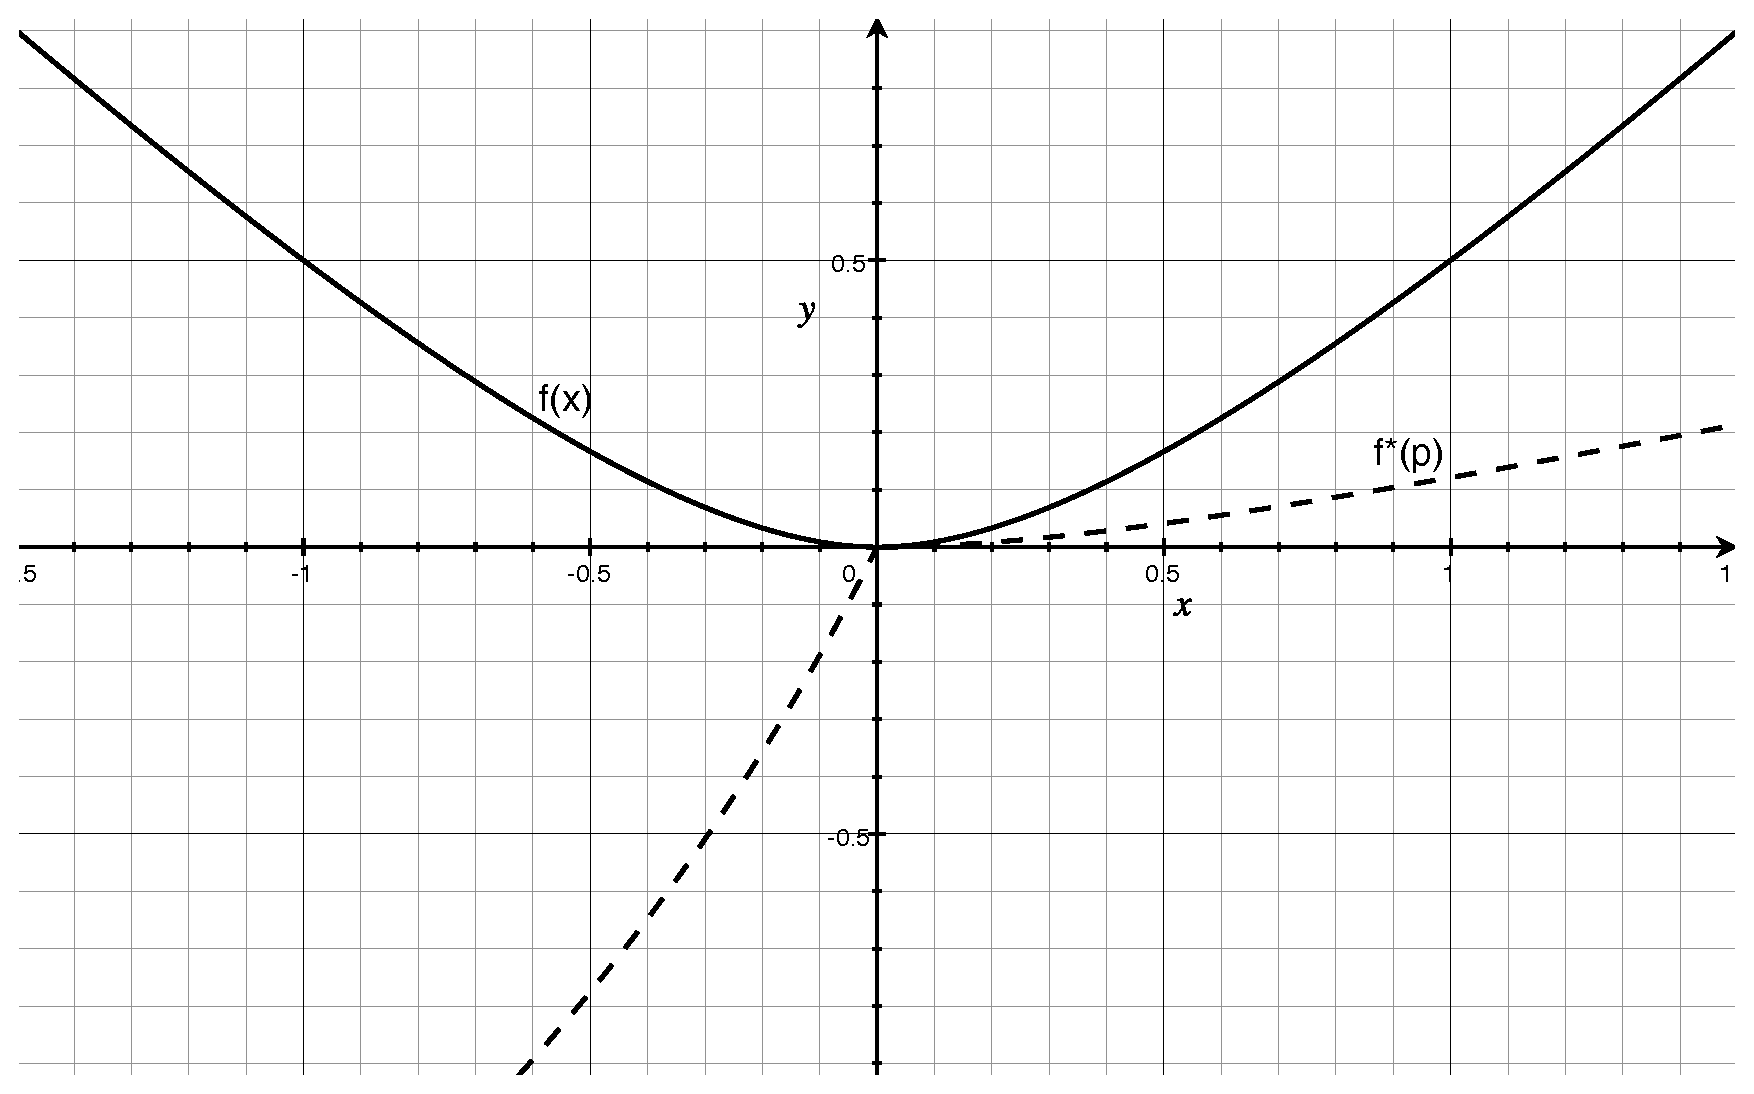
\includegraphics[width=\textwidth]{Problem_22_Plot.eps}
    \caption{Plot for Problem 22}
    \label{fig:problem_22_plot}
\end{figure}

\section*{23. One Nontrivial (but Enormously Instructive) Legendre Transform}
Consider the function $ f(x) $, which contains a parameter $ a \in \R $, and its Legendre transform $ f^*(p) $:
\begin{equation}
    f(x) = - \frac{1}{2} ax^2 + \frac{1}{4} x^4 \qquad f^*(p) = \min_x \{f(x) - px\}.
\end{equation}

Studying the Legendre transform $ f^*(p) $ is nontrivial, because depending on the value of $ a $, the function $ f(x) $ is not everywhere convex. Always keep in mind that the value of $ a $ might qualitatively change the results, so be careful about this.
\begin{itemize}
    \item[1.] Find any minima, maxima, and inflection points of $ f(x) $. For which values of $ a $ is the function always convex? Sketch $ f(x) $ for typical representative cases.
        \begin{problem}
            The derivative of the function is $ x^3 - ax $, so there are three critical points which we should examine, which are the roots $ x = 0 $ and $ x = \pm \sqrt{a} $. The second derivative is $ 3 x^2 - a $, so plugging these extrema in, we can see that $ 3 \left( \begin{cases} \pm \sqrt{a} \\ 0 \end{cases} \right)^2 - a = \begin{cases} 2a \\ -a \end{cases} $. When $ a > 0 $, $ \pm \sqrt{a} $ are minima, while $ 0 $ will be a maximum. When $ a < 0 $, $ 0 $ will now be a minimum, and the two extrema at $ \pm \sqrt{a} $ will become imaginary. Additionally, the two inflection points of $ f(x) $ are the roots of the second derivative: $ \pm \sqrt{\frac{a}{3}} $ and they also vanish for $ a < 0 $. It's clear that $ a < 0 $ makes the function always convex, since it will only have a single minimum and no inflection points. However, $ a > 0 $ will create two maxima, and the points between the inflection points will be concave while the rest of the function will be convex. See \Cref{fig:problem_23_1_plot} for some representative graphs.
        \end{problem}

        \begin{figure}[h]
            \centering
            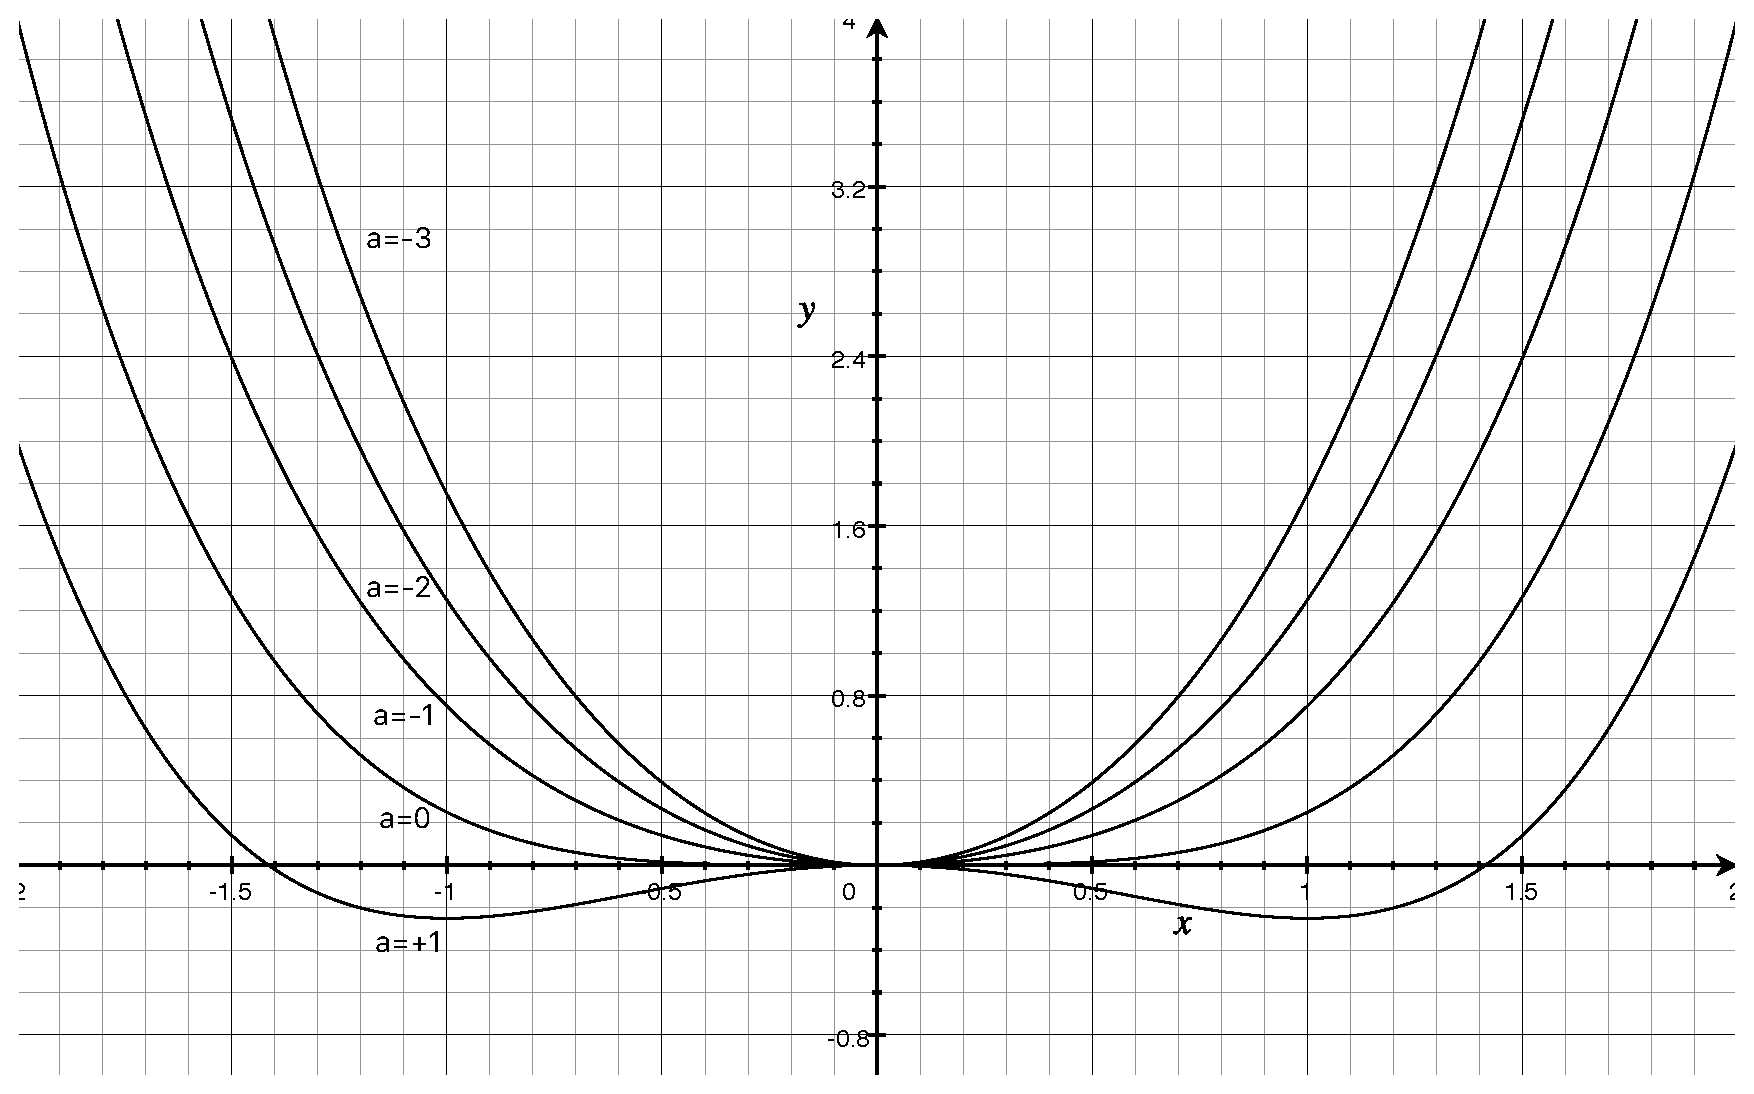
\includegraphics[width=\textwidth]{Problem_23_1_Plot.eps}
            \caption{Plot for Problem 23.1}
            \label{fig:problem_23_1_plot}
        \end{figure}

    \item[2.] In order to actually perform the Legendre transform, you need the equation that links $ p $ and $ x $. Find it.
        \begin{problem}
            I already did the derivative above. To minimize $ f(x) - px $, we require an $ x_0 $ such that
            \begin{equation}
                x_0^3 - a x_0 = p
            \end{equation}
        \end{problem}
        
    \item[3.] The graph of $ f^*(p) $ is the collection of points $ \{p, f^*(p)\} $. Neglecting for a moment the ``min'' prescription in the Legendre transform, let us consider the collection of points $ \{p(x), f(x) - p(x) x\} $, which you could view as a parametric representation of the graph of $ f^*(p) $ (with $ x $ being the parameter). Using your favorite plotting program, provide plots of that graph for representative values of $ a $. What happens when you tune $ a $ such that $ f(x) $ ceases to be convex? Which bits of the (possibly funny-looking) graph of $ f^*(p) $ will survive after applying the ``min'' in the Legendre transform that we have ignored so far? What therefore happens to the Legendre transform $ f^*(p) $ once $ f(x) $ deviates locally from convexity?
        \begin{problem}
            While my previous couple of plots have not used it, my favorite plotting program is Python. See \Cref{fig:problem_23_plots} for first, a plot of this parametric curve for a few values of $ a $, and second, for a demonstration of what makes the cut if you take the minimum or maximum values of the curve (although note that I did not faithfully represent the maximum for values of $ x $ outside the region where it's the same as the minimum, I couldn't think of a clever way to show it visually). When the function deviates from convexity, a maximizing transformation must be made rather than a minimization. This area corresponds to the region between the inflection points.
        \end{problem}
        \begin{figure}[h]
            \centering
            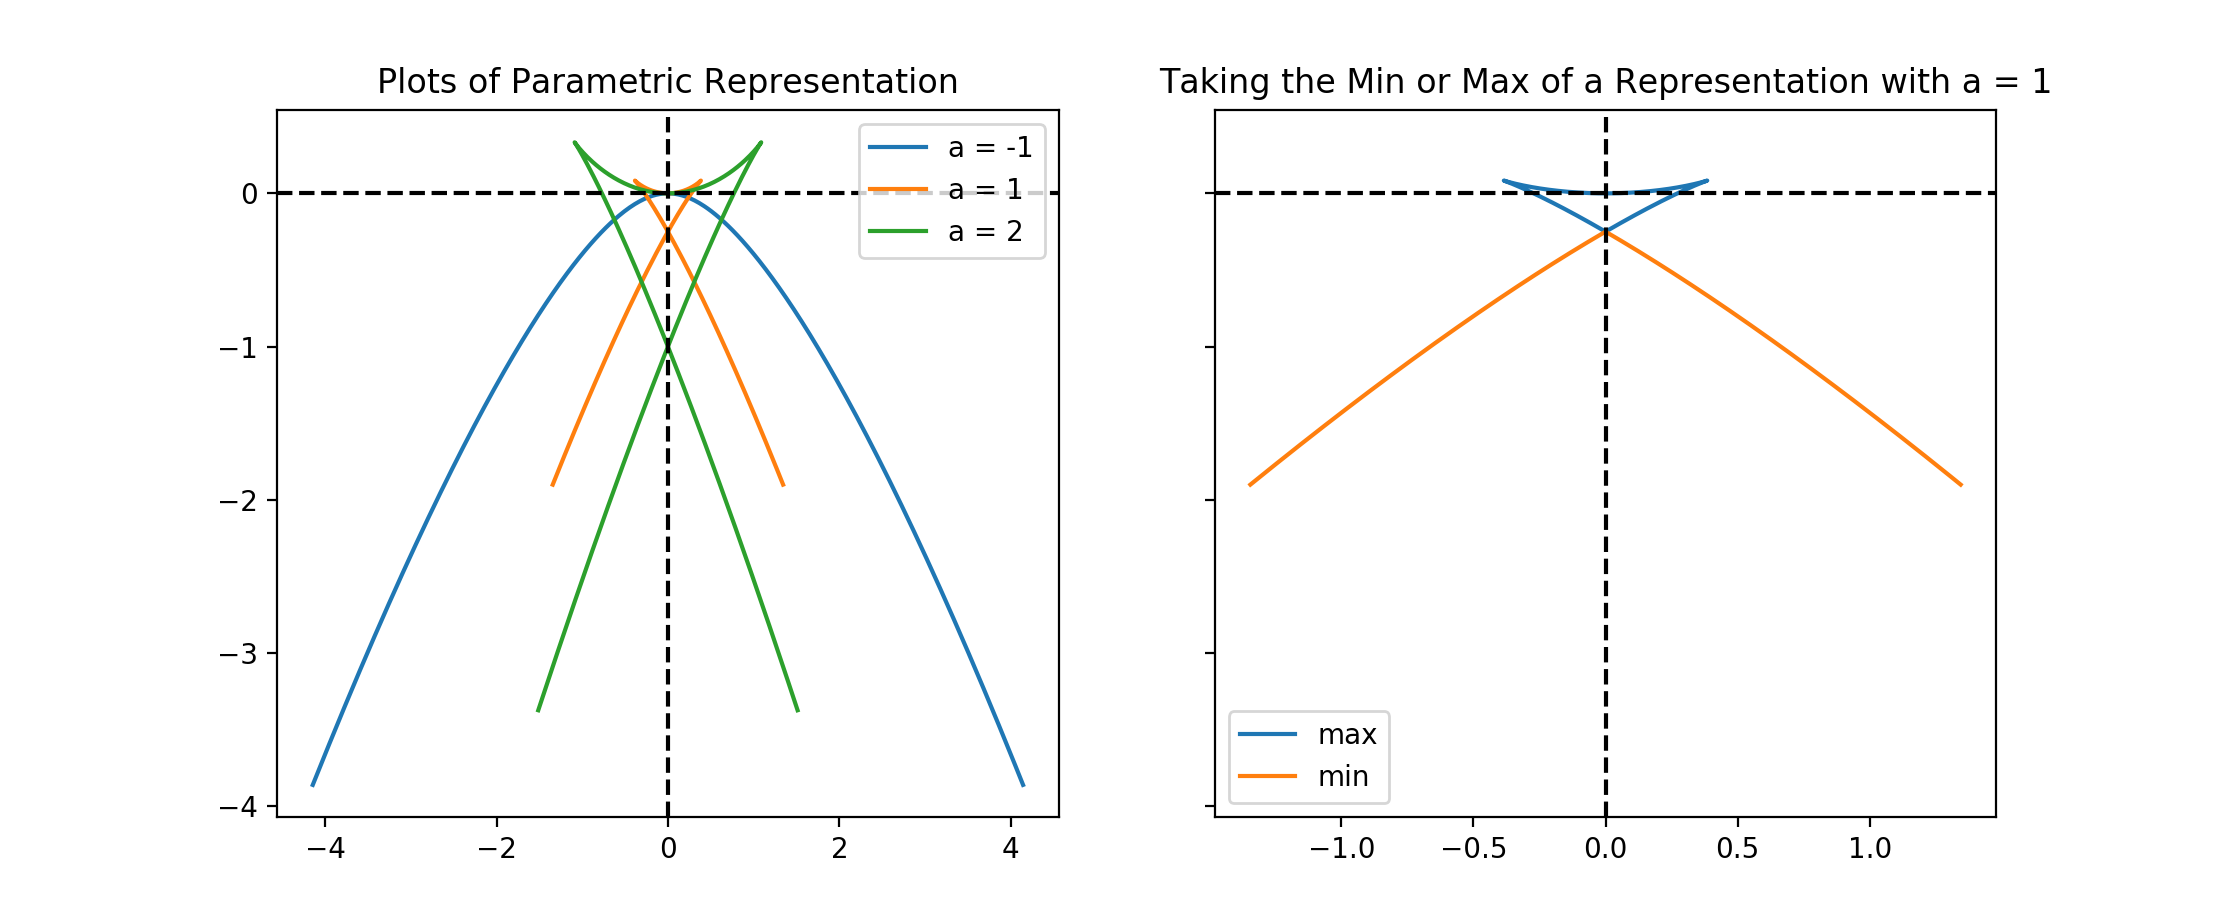
\includegraphics[width=\textwidth]{Problem_23_Plots.png}
            \caption{Plots for Problem 23.3}
            \label{fig:problem_23_plots}
        \end{figure}

    \item[4.] To get $ f^*(p) $, we need to solve the equation linking $ p $ and $ x $ for $ x $. Defining $ r^2 = \frac{4a}{3} $ and $ \cos(3 \alpha) = \frac{4p}{r^3} $, show (without using Mathematica or relatives!) that the three solutions $ \{x_0, x_1, x_2\} $ can be written as $ x_k = r \cos(\alpha + \frac{2 \pi}{3} k) $.
        \begin{problem}
            \begin{align}
                p(x) &= x^3 - ax \\
                \frac{r^3 \cos(3 \alpha)}{4} &= x^3 - \frac{3 r^2}{4} x \\
                \frac{r^3}{4} \left( 4 \cos[3](\alpha) - 3 \cos(\alpha) \right) &= \\
                (r \cos(\alpha))^3 - \frac{3 r^2}{4}r\cos(\alpha) &= x^3 - \frac{3 r^2}{4} x
            \end{align}
            Clearly, $ x = r \cos(\alpha) $ is a solution. If we factor it out, we will be left with some arbitrary quadratic:
            \begin{equation}
                (x - r \cos(\alpha))(x^2 + \beta x + \gamma) = x^3 - \frac{3r^2}{4} x
            \end{equation}
            Matching like powers of $ x $, we see that $ \beta = r \cos(\alpha) $ and $ \gamma = r^2 \cos[2](\alpha) - \frac{3}{4} r^2 $. The roots of this expression are
            \begin{equation}
                x = r\left( -\frac{1}{2} \cos(\alpha) \pm \frac{\sqrt{3}}{2} \sin(\alpha)  \right) = r \left( \cos(\frac{2 \pi}{3}) \cos(\alpha) \pm \sin(\frac{2 \pi}{3}) \sin(\alpha) \right) = \cos(\alpha \mp \frac{2 \pi}{3})
            \end{equation}
            by periodicity in the cosine, we can see that the given solutions are correct.
        \end{problem}
    \item[5.] Identify the three solutions with the three interesting branches of the Legendre transform which show up once $ f(x) $ is no longer convex. Feel free to use your favorite plotting program to do that; no formal proof is required.
        \begin{problem}
            If we solve our solutions for $ p $ and $ a $, we find that:
            \begin{equation}
                \alpha = \pm\frac{1}{3} \left( \arccos(\frac{3 \sqrt{3} p}{2 a^{3/2}}) + 2 \pi c \right) \qc c \in \Z
            \end{equation}
            Picking the positive solution and setting $ c = 0 $, we can then plug this into the three solutions and get regions corresponding to the graph in \Cref{fig:problem_23_5_plot}. Taking the other solution or a different value of $ c $ just cyclically rotates which region corresponds to the given solution. Additionally, in solving this, I took the positive root for $ r $ but I could have just as easily taken the negative root which would have introduced a negative sign into the argument of the arccosine. However, this reduces back to the original solutions if we choose a different branch of the arccosine, which is defined on the whole complex plane.
        \end{problem}
        \begin{figure}[h]
            \centering
            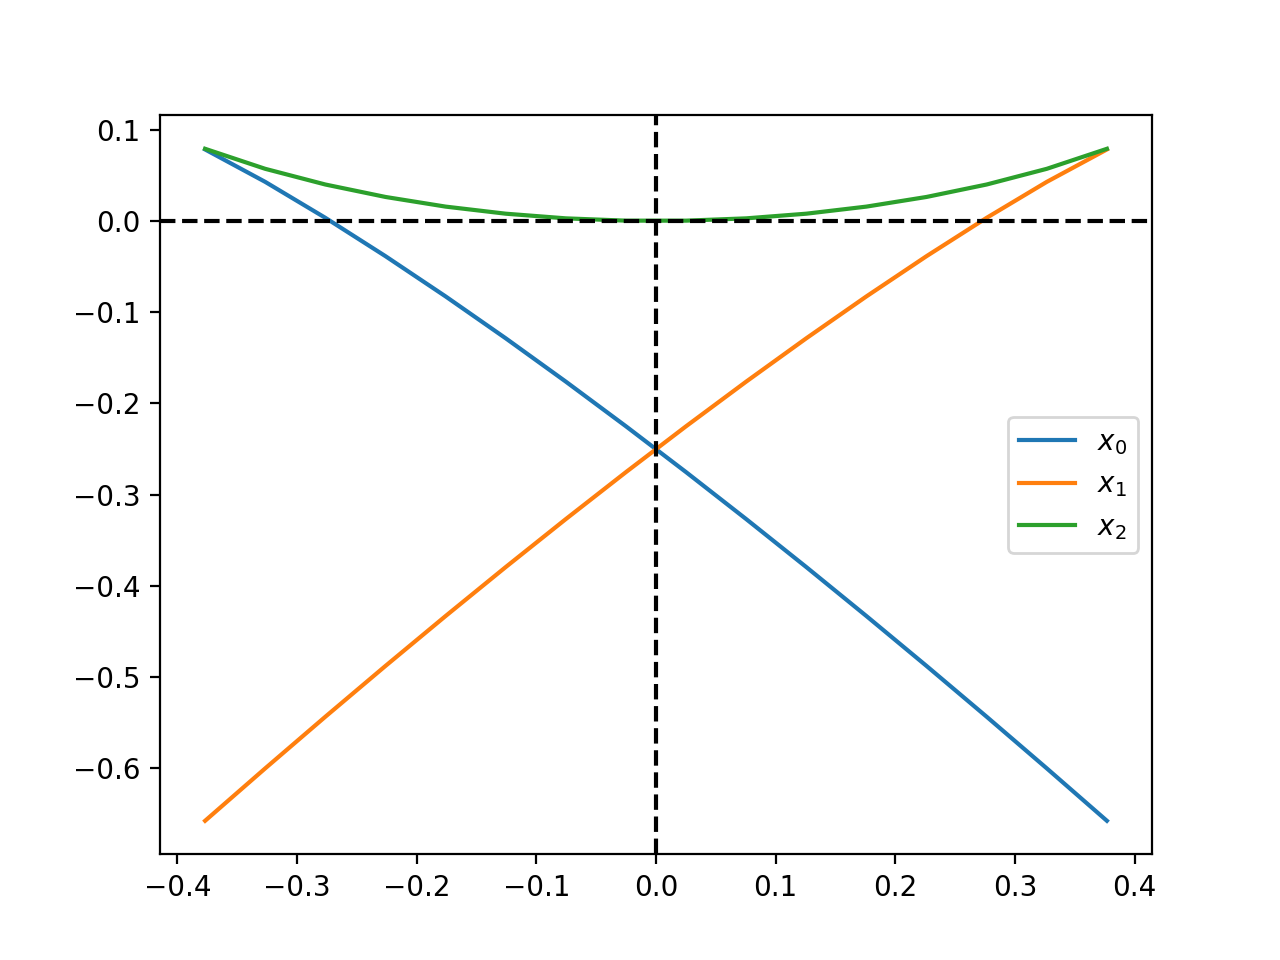
\includegraphics[width=\textwidth]{Problem_23_5_Plot.png}
            \caption{Plot for Problem 23.5 ($ a = 1 $)}
            \label{fig:problem_23_5_plot}
        \end{figure}
    \item[6.] What is $ f^*(0) $? And what is $ \lim_{p \to 0^+} {f^*}'(p) $ and $ \lim_{p \to 0^-} {f^*}'(p) $?
        \begin{problem}
            Clearly from the parametric plot there are two solutions at $ p = 0 $. One is where $ f^*(0) = 0 $ and the other (solving our solutions for $ p = 0 $ to get $ x_i = 0, \pm \sqrt{a} $, is $ f^*(0) = - \frac{a^2}{4} $. If we approach from the left, we use the first solution $ {f^*}'(0) = -x_0(0) = - \sqrt{a} $. From the right, I think we have to use $ {f^*}'(0) = - x_2(0) = 0 $, so I'm not quite sure what this is supposed to tell us, since I would expect both of these solutions to correspond to moving on the long arcs which give a zero at $ - \frac{a^2}{4} $ rather than the top solution. Technically we could also use the $ x_1 $ solution which would give $ \sqrt{\alpha} $ as the derivative, but I'm not sure which solution we're supposed to take as we approach from either side. Does this not depend on our choice of branch?
        \end{problem}
\end{itemize}

\end{document}
